\section{Absorption in superconductors and metals}\label{sec:15.4}

A dark photon of \SI{1}{meV} that is absorbed in aluminum gives up all of its energy but brings a momentum of only $m_\phi v \approx \SI{1}{\micro eV}$. To take up \SI{1}{meV}, an electron at the Fermi surface must change its momentum by at least $\omega/v_{\mathrm{F}} = \SI{0.15}{eV}$, a hundred thousand times more. A clean metal therefore cannot absorb the boson with one electron alone. A third body must take up the momentum: an impurity, which does so elastically, or a phonon, which carries off the momentum and part of the energy. \Cref{sec:10.7} expressed the rates of the dark photon and the axion-like particle through the optical conductivity $\sigma_1$ at the boson mass. In a metal below its interband threshold, about \SI{0.5}{eV} in aluminum~\cite[p.~4]{hochberg2016absorption}, that conductivity comes from the two third-body processes and from electron--electron collisions, a channel we name but do not size. Within a few gaps of the pair-breaking edge $2\Delta_{\mathrm{BCS}} = \SI{0.36}{meV}$ the superconducting state changes both third-body processes through the coherence factors of \cref{sec:7.2}: the phonon-assisted process carries the case-I factor and the impurity-assisted one the case-II factor. Both coherence factors follow from the structure of the current in the Nambu notation of \cref{sec:7.2}, and the phonon-assisted part reproduces the formula of Allen. In a clean singlet superconductor without spin--orbit coupling, the spin current, which absorbs the axion-like particle, breaks pairs without a third body.

\subsection{Impurity-assisted absorption}\label{sec:15.4-MB}

At $\vect{q} \to 0$ a dark photon, like a photon, couples to the total velocity $\op{\vect{V}}$ of the electrons, \cref{eq:6.5-HA}. In a metal below its interband threshold only the band that crosses the Fermi level contributes, and $\op{\vect{V}} = \sum_{\vect{k}\sigma}\vect{v}_{\vect{k}}\,c^\dagger_{\vect{k}\sigma}c_{\vect{k}\sigma}$ with the band velocity $\vect{v}_{\vect{k}} = \partial\xi_{\vect{k}}/\partial\vect{k}$. Time reversal makes $\xi_{-\vect{k}} = \xi_{\vect{k}}$, and therefore $\vect{v}_{-\vect{k}} = -\vect{v}_{\vect{k}}$. Relabeling $\vect{k} \to -\vect{k}$ in the spin-down term and writing the result with the Nambu spinors $\Psi_{\vect{k}}$ of \cref{eq:7.2-nambu} gives (\cref{app:D.40})
\begin{equation}
  \hat{\vect{e}}\cdot\op{\vect{V}} = \sum_{\vect{k}}(\hat{\vect{e}}\cdot\vect{v}_{\vect{k}})\,\Psi^\dagger_{\vect{k}}\Psi_{\vect{k}}
  = \sum_{\vect{k}}(\hat{\vect{e}}\cdot\vect{v}_{\vect{k}})\bigl(\gamma^\dagger_{\vect{k}1}\gamma_{\vect{k}1} - \gamma^\dagger_{\vect{k}2}\gamma_{\vect{k}2}\bigr) .
  \label{eq:15.4-Vnambu}
\end{equation}
The density is the matrix $\boldsymbol{\eta}$ in Nambu space; the uniform current is the unit matrix. The difference between the two matrices comes from the sign of the velocity under $\vect{k} \to -\vect{k}$, which the density, an even function of $\vect{k}$, does not have. The unit matrix commutes with $h_{\vect{k}}$, so the current commutes with $H_{\mathrm{MF}}$, and in the quasiparticle basis it only counts: $\gamma^\dagger_{\vect{k}1}$ carries the velocity $\vect{v}_{\vect{k}}$ of its electron $(\vect{k}\!\uparrow)$ and $\gamma^\dagger_{\vect{k}2}$ the velocity $\vect{v}_{-\vect{k}}$ of $(-\vect{k}\!\downarrow)$. The current creates no pairs. A clean BCS superconductor therefore absorbs nothing at $\vect{q} \to 0$ and $\omega > 0$, and the whole intraband weight of the f-sum rule lies at $\omega = 0$, as the supercurrent. The clean normal metal behaves the same way, with a Drude peak of zero width. This intraband weight is $(\pi/2)(\omega_p^{\mathrm{intra}})^2$, with the intraband plasma frequency
\begin{equation}
  (\omega_p^{\mathrm{intra}})^2 = 2e^2\,\mathcal{N}_{\mathrm{F}}\,\langle(\hat{\vect{e}}\cdot\vect{v})^2\rangle_{\mathrm{FS}} ,
  \label{eq:15.4-wp}
\end{equation}
where $\langle\dots\rangle_{\mathrm{FS}}$ is the average over the Fermi surface and the factor 2 counts the spins. For free electrons the intraband plasma frequency is $\omega_p$ of \cref{sec:4.3}, \SI{15.78}{eV} for the three valence electrons of aluminum; the computed bands of aluminum give \SI{12.29}{eV}~\cite[Table~IV]{savrasov1996electron}, which we use.

An impurity breaks the conservation of momentum, and with it the commutation of the current with $H_{\mathrm{MF}}$. The one-electron eigenstates $\alpha$ of the disordered metal have energies $\xi_\alpha$ and no definite momentum, but time reversal still pairs each with a partner $\bar\alpha$ of the same energy, and for nonmagnetic disorder the paired state is built from $(\alpha\!\uparrow, \bar\alpha\!\downarrow)$ with the same gap (\cref{sec:15.3}). The current acquires matrix elements $\langle\alpha|\hat{\vect{e}}\cdot\op{\vect{v}}|\beta\rangle$ between different states, and since it is odd under time reversal it is still the unit matrix in the Nambu space of $(\alpha, \bar\alpha)$. The pair-creation amplitude of the current then carries $u^{\mathrm{B}}_\alpha v^{\mathrm{B}}_\beta - v^{\mathrm{B}}_\alpha u^{\mathrm{B}}_\beta$, the case-II factor of \cref{eq:7.2-coh}, which vanishes for two quasiparticles at the gap edge (\cref{app:D.40}). In the dirty limit the relaxation rate $\gamma_{\mathrm{rel}} = v_{\mathrm{F}}/\mathfrak{l}_e$ far exceeds $\Delta_{\mathrm{BCS}}$ ($\mathfrak{l}_e \ll \xi_{\mathrm{coh}}$, \cref{sec:15.3}), and the squared matrix elements change only over energies of order $\gamma_{\mathrm{rel}}$. Over the few $\Delta_{\mathrm{BCS}}$ where the coherence factors matter, the squared matrix elements are constant, and $\xi_\alpha$ and $\xi_\beta$ are independent. The ratio of the superconducting to the normal absorption is then the case-II integral of \cref{eq:7.2-pairspec}:
\begin{keyresult}[Impurity-assisted absorption (Mattis--Bardeen)]
\begin{equation}
  \begin{gathered}
  \sigma_1^{\mathrm{MB}}(\omega) = \sigma_n(\omega)\,\mathfrak{g}_{\mathrm{II}}\Bigl(\frac{\omega}{\Delta_{\mathrm{BCS}}}\Bigr), \qquad
  \sigma_n(\omega) = \frac{\sigma_{\mathrm{dc}}\,\gamma_{\mathrm{rel}}^2}{\omega^2 + \gamma_{\mathrm{rel}}^2} , \\
  \mathfrak{g}_{\mathrm{II}}(y) = \Bigl(1 + \frac2y\Bigr)\mathrm{E}(k) - \frac4y\,\mathrm{K}(k) ,
  \end{gathered}
  \label{eq:15.4-MB}
\end{equation}
for $\omega \ge 2\Delta_{\mathrm{BCS}}$ and $\gamma_{\mathrm{rel}} \gg \Delta_{\mathrm{BCS}}$, with $\sigma_n$ the Drude conductivity of the normal metal, $\sigma_{\mathrm{dc}}$ its dc value, and $\mathrm{K}$, $\mathrm{E}$ the complete elliptic integrals of the modulus $k = (y - 2)/(y + 2)$ of \cref{eq:15.1-gI} (\cref{eq:D.40-g}).
\end{keyresult}
\noindent \Cref{eq:15.4-MB} is the absorption of light by a superconductor that Mattis and Bardeen found~\cite{mattis1958theory}; \cref{sec:7.2} met its zero-temperature ratio as the case-II pair-creation spectrum. The function $\mathfrak{g}_{\mathrm{II}}$ starts from zero at the edge, is 0.67 at $4\Delta_{\mathrm{BCS}}$ and comes within \SI{10}{\percent} of one at $8.1\,\Delta_{\mathrm{BCS}}$; its case-I partner $\mathfrak{g}_{\mathrm{I}}$ of \cref{sec:15.1} has the same closed form with $4/(y + 2)$ in place of $4/y$. No ladder of the pair field corrects \cref{eq:15.4-MB}. In the conserving response \cref{eq:7.2-Rc} the current would couple to the amplitude and phase channels through bubbles that pair one odd factor $\vect{v}$ with an even pair vertex, and these bubbles vanish. The bubble of independent quasiparticles in the exact impurity states is already the conserving response at $\vect{q} \to 0$, and through the continuity equation it is the long-wavelength limit of the density response of \cref{sec:15.1}.

Impurity-assisted absorption is large in a film. The \SI{50}{nm} aluminum film of \cref{we:15-film}, with $\mathfrak{l}_e = \SI{50}{nm}$, has $\gamma_{\mathrm{rel}} = \SI{26.7}{meV}$, 148 gaps, and with the free-electron plasma frequency its dc conductivity is $\sigma_{\mathrm{dc}} = \omega_p^2/\gamma_{\mathrm{rel}} = \SI{9.35e3}{eV}$, a residual resistivity of \SI{0.80}{\micro\ohm.cm}. At \SI{1}{meV} the paired film absorbs with $\sigma_1^{\mathrm{MB}} = \SI{7.56e3}{eV}$, $1.4\times10^6$ times the phonon-assisted value derived next. Intrinsic absorption dominates only in a pure sample, as Hochberg, Lin and Zurek assumed~\cite{hochberg2016absorption}, and in a film the rate follows the residual resistivity of the sample, not a property of aluminum.

\subsection{Phonon-assisted absorption}\label{sec:15.4-holstein}

In a pure crystal the third body is a phonon. The absorption is then of second order, with one current vertex and one electron--phonon vertex, as for phonon-assisted absorption across the gap of silicon (\cref{sec:6.5}), and the phonon carries the momentum that the electrons need. At \SI{1}{meV} in aluminum the phonon has at most $\omega - 2\Delta_{\mathrm{BCS}} = \SI{0.64}{meV}$. With the sound speeds along [100] from the zero-temperature elastic constants, $c_{\mathrm{LA}} = \SI{6.47}{km.s^{-1}}$ and $c_{\mathrm{TA}} = (C_{44}/\rho)^{1/2} = \SI{3.40}{km.s^{-1}}$ for $C_{44} = \SI{31.6}{GPa}$~\cite[Table~2]{malica2020quasi} and $\rho = \SI{2.73}{g.cm^{-3}}$, that is a momentum of at most 29.7 or \SI{56.4}{eV}. The smaller value is two hundred times the \SI{0.15}{eV} that the electrons need, and the larger is 61 times less than $k_{\mathrm{F}} = \SI{3.45}{keV}$, so only long-wavelength acoustic phonons take part near the edge. In a superconductor the question is which coherence factor the final pair carries, and the Nambu form \cref{eq:15.4-Vnambu} answers it exactly.

Take the electron--phonon Hamiltonian \cref{eq:A.6-Hep} restricted to the band at the Fermi level, with the vertex $g_\nu(\vect{k},\vect{Q})$, and the final states with one quasiparticle in $(\vect{k}+\vect{Q}\!\uparrow)$, one in $(-\vect{k}\!\downarrow)$ and an emitted phonon $(-\vect{Q},\nu)$. The second-order amplitude has the two time orderings of \cref{eq:13.2-T}, with the current in place of the density. The current is diagonal in the quasiparticle basis, so every intermediate state reached by the current is the state it acted on. The sum over intermediate states collapses, and the amplitude is the matrix element of the phonon vertex times the change of the current eigenvalue, $J_f - J_i$, divided by $-\omega$ (\cref{eq:D.40-T}). The ground state carries no current, and by \cref{eq:15.4-Vnambu} the final pair carries $\hat{\vect{e}}\cdot(\vect{v}_{\vect{k}+\vect{Q}} - \vect{v}_{\vect{k}})$. The phonon vertex creates the pair through its spin-up and spin-down terms, as the density does in \cref{eq:7.2-coh}. With the phase convention in which time reversal gives $g_\nu(-\vect{k}-\vect{Q},\vect{Q}) = g_\nu(\vect{k},\vect{Q})$,
\begin{keyresult}[Phonon-assisted amplitude in a superconductor]
\begin{equation}
  T_{fi} = -\frac{\hat{\vect{e}}\cdot(\vect{v}_{\vect{k}+\vect{Q}} - \vect{v}_{\vect{k}})}{\omega}\,\frac{1}{\sqrt N}\,g_\nu(\vect{k},\vect{Q})\,\bigl(u^{\mathrm{B}}_{\vect{k}+\vect{Q}}v^{\mathrm{B}}_{\vect{k}} + v^{\mathrm{B}}_{\vect{k}+\vect{Q}}u^{\mathrm{B}}_{\vect{k}}\bigr) ,
  \label{eq:15.4-T}
\end{equation}
for $|f\rangle = \gamma^\dagger_{\vect{k}+\vect{Q},1}\gamma^\dagger_{\vect{k}2}b^\dagger_{-\vect{Q}\nu}|\mathrm{BCS}\rangle$ at $T = 0$, with $\omega = E_{\vect{k}+\vect{Q}} + E_{\vect{k}} + \omega_{\vect{Q}\nu}$ and $N$ the number of unit cells.
\end{keyresult}
\noindent No intermediate state needs to be far from the energy shell. The only input is that the current commutes with the mean-field Hamiltonian, and the result holds for any $\omega$ and any phonon energy. The current supplies only the velocity difference, the factor that suppresses forward scattering. The pair itself is created by the phonon, through a vertex even under time reversal, and so it carries the case-I factor of the density. Phonon-assisted absorption has the coherence factor of the density, impurity-assisted absorption that of the current. The same steps with the density in place of the current give zero, because the eigenvalue of the density at $\vect{q} = 0$ is the conserved electron number, as in \cref{eq:13.2-q0}.

The conductivity follows from the absorbed power as in \cref{sec:6.5},
\begin{equation*}
  \sigma_1 = \frac{\pi e^2}{\omega\Vol}\sum_f|T_{fi}|^2\,\delta(E_f - E_i - \omega) .
\end{equation*}
The band velocity and the vertex change across the Fermi surface on scales of eV, whereas $\xi_{\vect{k}}$ and $\xi_{\vect{k}+\vect{Q}}$ range only over $\omega$. The sum over $\vect{k}$ and $\vect{Q}$ therefore splits into an average over the Fermi surface and independent integrals over the two energies. The integrals give the pair spectrum $2x\,\mathfrak{g}_{\mathrm{I}}(x/\Delta_{\mathrm{BCS}})$ at the pair energy $x = \omega - \omega_{\vect{Q}\nu}$, the case-I integral of \cref{eq:7.2-pairspec}. The average defines the transport Eliashberg function,
\begin{equation}
  \alpha^2F_{\mathrm{tr}}(\omega) = \frac{1}{2\langle(\hat{\vect{e}}\cdot\vect{v})^2\rangle_{\mathrm{FS}}\,\mathcal{N}_{\mathrm{F}}\Omega\,N^2}\sum_{\vect{k}\vect{Q}\nu}|g_\nu(\vect{k},\vect{Q})|^2\bigl[\hat{\vect{e}}\cdot(\vect{v}_{\vect{k}+\vect{Q}} - \vect{v}_{\vect{k}})\bigr]^2\delta(\xi_{\vect{k}})\,\delta(\xi_{\vect{k}+\vect{Q}})\,\delta(\omega - \omega_{\vect{Q}\nu}) ,
  \label{eq:15.4-a2Ftr}
\end{equation}
with $\Omega$ the volume of the unit cell, so that $\Vol = N\Omega$. This transport function is the Eliashberg function of \cref{eq:6.4-a2F} with each pair of Fermi-surface points weighted by the change of the velocity. For a spherical Fermi surface in a cubic crystal the weight averages to $\langle[\hat{\vect{e}}\cdot(\vect{v}' - \vect{v})]^2\rangle = 2(1 - \cos\theta_{\vect{k}\vect{k}+\vect{Q}})\langle(\hat{\vect{e}}\cdot\vect{v})^2\rangle_{\mathrm{FS}}$, and with the factor $\frac12$ of the definition the weight is $1 - \cos\theta_{\vect{k}\vect{k}+\vect{Q}}$, which removes forward scattering. The transport coupling constant is $\lambda_{\mathrm{tr}} = 2\int\dd\omega\,\alpha^2F_{\mathrm{tr}}(\omega)/\omega$. Inserting \cref{eq:15.4-wp} gives (\cref{app:D.40})
\begin{keyresult}[Phonon-assisted (Holstein) absorption]
\begin{equation}
  \begin{gathered}
  \sigma_1^{\mathrm{S}}(\omega) = \frac{(\omega_p^{\mathrm{intra}})^2}{\omega^2}\,\frac{2\pi}{\omega}\int_0^{\omega - 2\Delta_{\mathrm{BCS}}}\dd\omega'\,\alpha^2F_{\mathrm{tr}}(\omega')\,(\omega - \omega')\,\mathfrak{g}_{\mathrm{I}}\Bigl(\frac{\omega - \omega'}{\Delta_{\mathrm{BCS}}}\Bigr) , \\
  \sigma_1^{\mathrm{N}}(\omega) = \frac{(\omega_p^{\mathrm{intra}})^2}{\omega^2}\,\gamma_{\mathrm{H}}(\omega), \qquad
  \gamma_{\mathrm{H}}(\omega) = \frac{2\pi}{\omega}\int_0^{\omega}\dd\omega'\,(\omega - \omega')\,\alpha^2F_{\mathrm{tr}}(\omega') ,
  \end{gathered}
  \label{eq:15.4-holstein}
\end{equation}
for the superconductor and the normal metal at $T = 0$, $\omega$ below the interband threshold and above the impurity rate.
\end{keyresult}
\noindent The normal-metal form is Allen's formula for the phonon-assisted optical conductivity~\cite{allen1971electron}, as quoted by Hochberg, Lin and Zurek~\cite[Eqs.~(13), (16)]{hochberg2016absorption}: a Drude conductivity at $\omega \gg \gamma_{\mathrm{H}}$ with the frequency-dependent scattering rate $\gamma_{\mathrm{H}}(\omega)$ of an electron that absorbs $\omega$ and emits a phonon. The superconducting form, with its case-I factor and the bound $\omega' \le \omega - 2\Delta_{\mathrm{BCS}}$, is also Allen's~\cite[Eq.~(17)]{hochberg2016absorption}, and it holds for intermediate states on shell as well. Two of its hypotheses can be sized. The pair created by the phonon is not dressed by the ladder of \cref{eq:7.2-Rc}. The ladder correction is of relative order $(\Delta_{\mathrm{BCS}}/v_{\mathrm{F}}Q)^2$ at the phonon momentum $Q$ (\cref{sec:7.2}); averaged over the integrand of \cref{eq:15.4-holstein} with the $\omega'^4$ law below, it is $4\times10^{-4}$ at $\omega = 2.2\,\Delta_{\mathrm{BCS}}$ ($2.6\times10^{-4}$ for the most energetic phonon) and $1.4\times10^{-6}$ at \SI{1}{meV}. At millikelvin temperatures there are no thermal phonons to absorb, and thermal quasiparticles are suppressed by $\ee^{-\Delta_{\mathrm{BCS}}/T}$ (\cref{sec:7.2}).

The dark-matter literature evaluates \cref{eq:15.4-holstein} with a Debye transport function, $\alpha^2F_{\mathrm{tr}}(\omega') = 2\lambda_{\mathrm{tr}}\omega'^4/\omega_{\mathrm{D}}^4$ below $\omega_{\mathrm{D}}$, which carries the coupling $\lambda_{\mathrm{tr}}$. The fourth power is that of long-wavelength longitudinal phonons: $\alpha^2F$ grows as $\omega'^2$ (\cref{sec:6.4}), and the transport weight $1 - \cos\theta \propto Q^2$ adds two more powers. The rate is then $\gamma_{\mathrm{H}} = (2\pi/15)\lambda_{\mathrm{tr}}\omega^5/\omega_{\mathrm{D}}^4$ below $\omega_{\mathrm{D}}$, and above it $\gamma_{\mathrm{H}} = (4\pi/5)\lambda_{\mathrm{tr}}\omega_{\mathrm{D}}(1 - 5\omega_{\mathrm{D}}/6\omega)$, the result of Ref.~\cite[Eq.~(16)]{hochberg2016absorption}, and the ratio of the two lines of \cref{eq:15.4-holstein} is their Eq.~(17) (\cref{app:D.40}). Below $\omega_{\mathrm{D}}$ that ratio depends only on the power law, not on $\lambda_{\mathrm{tr}}$ or $\omega_{\mathrm{D}}$. For aluminum we take $\omega_{\mathrm{D}} = \SI{37}{meV}$~\cite{hochberg2016absorption} and $\lambda_{\mathrm{tr}} = 0.39$, the value that Savrasov and Savrasov extract from the measured resistivity with their computed plasma frequency~\cite[Table~IV]{savrasov1996electron}; their linear-response calculation gives 0.37. \Cref{lim:15.4a} compares the superconducting rate with the normal-metal formula.

\begin{limitbox}[Phonon-assisted absorption: the normal-metal limit][lim:15.4a]
Phonon-assisted absorption of a superconductor, \cref{eq:15.4-holstein} with $\alpha^2F_{\mathrm{tr}} = 2\lambda_{\mathrm{tr}}\omega'^4/\omega_{\mathrm{D}}^4$~\cite[Eqs.~(13), (16), (17)]{hochberg2016absorption}, following Allen~\cite{allen1971electron} as quoted there; for $\omega \gg \Delta_{\mathrm{BCS}}$ it becomes the normal-metal formula $\sigma_1^{\mathrm{N}} = (\omega_p^{\mathrm{intra}})^2\gamma_{\mathrm{H}}/\omega^2$.
\par\smallskip
{\centering
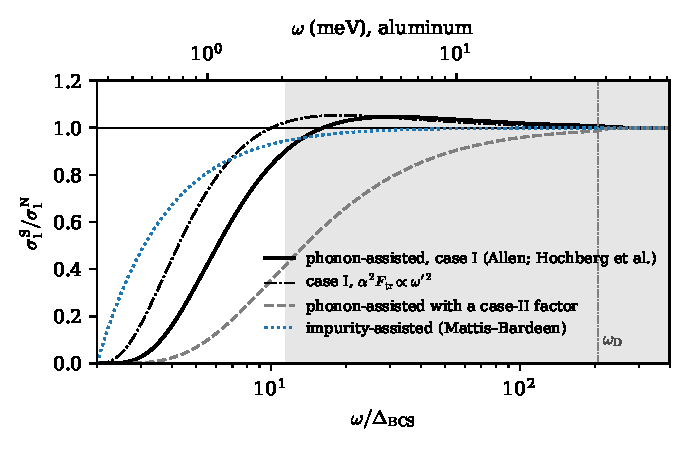
\includegraphics[width=0.85\linewidth]{figures/ch15/limit15_4a.pdf}
\captionof{figure}{Phonon-assisted conductivity of a superconductor over that of the normal metal, $\sigma_1^{\mathrm{S}}/\sigma_1^{\mathrm{N}}$, against $\omega/\Delta_{\mathrm{BCS}}$ (top axis: $\omega$ for aluminum, $\Delta_{\mathrm{BCS}} = \SI{0.18}{meV}$), at $T = 0$. Black: \cref{eq:15.4-holstein} with the case-I factor and the Debye law $\alpha^2F_{\mathrm{tr}} \propto \omega'^4$, which is the ratio of Hochberg, Lin and Zurek and, below $\omega_{\mathrm{D}}$ (dash-dotted vertical line, \SI{37}{meV}), independent of $\lambda_{\mathrm{tr}}$ and $\omega_{\mathrm{D}}$; dash-dotted: the same with the softer law $\alpha^2F_{\mathrm{tr}} \propto \omega'^2$, a test of the shape. Thin line at one: the normal-metal formula of Allen. Dashed: the phonon-assisted integral with the case-II factor in place of the case-I factor, for comparison. Dotted: impurity-assisted absorption in the dirty limit, $\mathfrak{g}_{\mathrm{II}}(\omega/\Delta_{\mathrm{BCS}})$, \cref{eq:15.4-MB}. Gray: the case-I result within \SI{10}{\percent} of the normal-metal formula, $\omega \ge 11.4\,\Delta_{\mathrm{BCS}}$ (\SI{2.05}{meV}).}\label{fig:15-limit-holstein}
\par}
\smallskip
Below $11.4\,\Delta_{\mathrm{BCS}}$ the normal-metal formula overstates the rate, by a factor of 2.4 at \SI{1}{meV} and without bound toward the edge, where the superconducting rate falls as $(\omega - 2\Delta_{\mathrm{BCS}})^5$; there the result also depends on the shape of $\alpha^2F_{\mathrm{tr}}$ below a few meV (0.42 or 0.73 of the normal value at \SI{1}{meV} for the two laws).
\end{limitbox}

The gap removes the absorption near the edge for a reason of phase space, not of coherence. The case-I factor is largest at the edge, where $\mathfrak{g}_{\mathrm{I}} = \pi/2$, but a phonon of energy $\omega'$ is available only up to $\omega - 2\Delta_{\mathrm{BCS}}$. Since $\alpha^2F_{\mathrm{tr}}$ grows as $\omega'^4$, the gap removes the most energetic phonons, which carry most of the weight. Above $16\,\Delta_{\mathrm{BCS}}$ the pile-up of the case-I factor dominates and the superconductor absorbs slightly more than the normal metal, by at most \SI{4.7}{\percent}, at $31\,\Delta_{\mathrm{BCS}}$. Had the pair carried the case-II factor of impurity-assisted absorption, the rate would reach \SI{90}{\percent} of the normal value only at $54\,\Delta_{\mathrm{BCS}}$. \Cref{fig:15-absorption}a shows the two processes on an absolute scale. The phonon-assisted conductivity of the normal metal grows as $\omega^3$ up to $\omega_{\mathrm{D}}$ and falls as $\omega^{-2}$ above. The impurity-assisted conductivity of the \SI{50}{nm} film, however, is flat up to $\gamma_{\mathrm{rel}}$ and stays above the phonon-assisted conductivity at every energy of the figure, by a factor of 1.6 at \SI{0.1}{eV} and 1.3 at \SI{0.3}{eV}.

\begin{figure}[tbp]
  \centering
  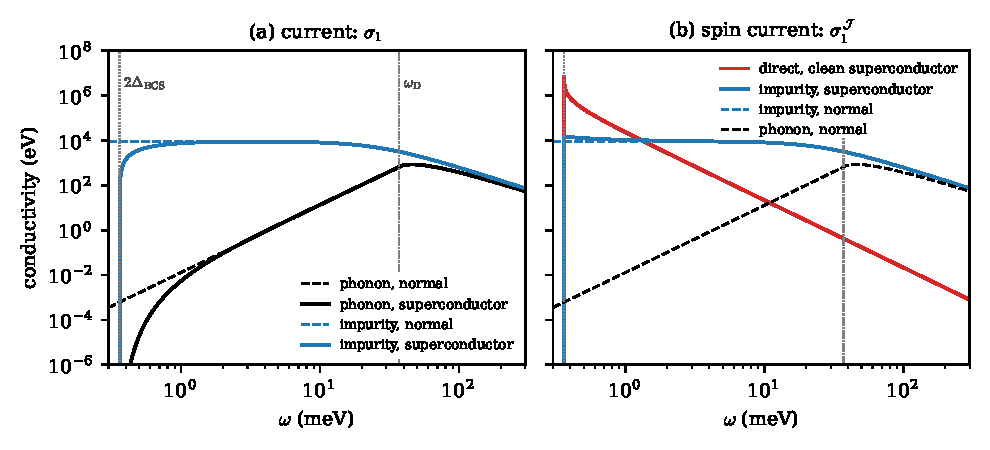
\includegraphics[width=\linewidth]{figures/ch15/fig15_3.pdf}
  \caption{Absorption of a uniform field by aluminum at $T = 0$, against the boson energy $\omega$, with $\Delta_{\mathrm{BCS}} = \SI{0.18}{meV}$ (dotted vertical line at $2\Delta_{\mathrm{BCS}}$) and the computed intraband plasma frequency \SI{12.29}{eV}. (a) Optical conductivity $\sigma_1$, which sets the rates of the dark photon. Black: phonon-assisted, \cref{eq:15.4-holstein}, in the normal metal (dashed) and the superconductor (solid), with the Debye transport function, $\lambda_{\mathrm{tr}} = 0.39$ and $\omega_{\mathrm{D}} = \SI{37}{meV}$ (dash-dotted vertical line). Blue: impurity-assisted, the Drude conductivity of the normal metal (dashed) and the Mattis--Bardeen conductivity of the superconductor (solid), \cref{eq:15.4-MB}, for the \SI{50}{nm} film of \cref{we:15-film} (mean free path \SI{50}{nm}, $\gamma_{\mathrm{rel}} = \SI{26.7}{meV}$, free-electron plasma frequency \SI{15.78}{eV} in its Drude conductivity). (b) Spin-current conductivity $\sigma_1^{\mathcal{J}}$, which sets the rate of the axion-like particle, normalized to equal $\sigma_1$ in the normal metal. Red: direct pair breaking in the clean superconductor, \cref{eq:15.4-sJ} with the quasiparticle factor $1/(1 + \lambda_{\mathrm{ep}}) = 0.70$. Blue: impurity-assisted, with the case-I factor in the superconductor (solid) and the Drude form in the normal metal (dashed), same mean free path. Black dashed: the phonon-assisted conductivity of the normal metal, for reference. Interband absorption, above about \SI{0.5}{eV}, is not included.}
  \label{fig:15-absorption}
\end{figure}

\begin{workedexample}{The Holstein onset in aluminum}\label{we:15-holstein}
A dark photon of $m_\phi = \SI{1}{meV}$, $5.56\,\Delta_{\mathrm{BCS}}$, is absorbed by pure aluminum with one phonon. The Debye form gives the normal-metal scattering rate $\gamma_{\mathrm{H}} = (2\pi/15)\lambda_{\mathrm{tr}}\omega^5/\omega_{\mathrm{D}}^4 = \SI{8.72e-11}{eV}$, and with $\omega_p^{\mathrm{intra}} = \SI{12.29}{eV}$ the normal-metal conductivity is $\sigma_1^{\mathrm{N}} = (\omega_p^{\mathrm{intra}})^2\gamma_{\mathrm{H}}/\omega^2 = \SI{0.0132}{eV}$. The superconductor has $\sigma_1^{\mathrm{S}}/\sigma_1^{\mathrm{N}} = 0.421$, so $\sigma_1^{\mathrm{S}} = \SI{5.54e-3}{eV}$.

Close to the edge the integral of \cref{eq:15.4-holstein} simplifies. For $\omega - 2\Delta_{\mathrm{BCS}} \ll \Delta_{\mathrm{BCS}}$ the pair energy $\omega - \omega'$ stays near $2\Delta_{\mathrm{BCS}}$ and $\mathfrak{g}_{\mathrm{I}}$ near $\pi/2$, and
\begin{equation*}
  \sigma_1^{\mathrm{S}} \simeq \frac{(\omega_p^{\mathrm{intra}})^2}{\omega^2}\,\frac{2\pi}{\omega}\,\frac{2\lambda_{\mathrm{tr}}}{\omega_{\mathrm{D}}^4}\,\frac{\pi}{2}\,2\Delta_{\mathrm{BCS}}\,\frac{(\omega - 2\Delta_{\mathrm{BCS}})^5}{5} .
\end{equation*}
At $\omega = 2.05$ and $2.5\,\Delta_{\mathrm{BCS}}$ this approximation is within 0.2 and \SI{2.1}{\percent} of the full integral. At $2.2\,\Delta_{\mathrm{BCS}}$ the superconductor absorbs with $\sigma_1^{\mathrm{S}} = \SI{4.4e-8}{eV}$, against $\SI{8.2e-4}{eV}$ for the normal metal: in practice the onset lies above $2\Delta_{\mathrm{BCS}}$.

The rate needs the loss function, $L = \varepsilon_2/|\varepsilon|^2$ in \cref{eq:10.7-dp}. At \SI{1}{meV} the condensate dominates $\varepsilon$: in the clean superconductor at $T = 0$ the imaginary conductivity is $\sigma_2 = (\omega_p^{\mathrm{intra}})^2/\omega$, and $\varepsilon_1 = 1 - \sigma_2/\omega = -1.51\times10^8$. The in-medium factor $1/|\varepsilon|^2$ is $4.4\times10^{-17}$, and $L = \sigma_1^{\mathrm{S}}\omega^3/(\omega_p^{\mathrm{intra}})^4 = 2.43\times10^{-16}$. With $\rho_\chi = \SI{0.3}{GeV.cm^{-3}}$ and $\rho_T = \SI{2.70}{g.cm^{-3}}$, \cref{eq:10.7-dp} gives $1.29\times10^{18}\,\zeta^2$ events per kilogram-year, and three events need $\zeta = 1.5\times10^{-9}$. The normal-metal formula would claim $9.9\times10^{-10}$. In the \SI{50}{nm} film of \cref{we:15-film} the impurity-assisted conductivity at the same mass is $1.4\times10^6$ times larger, and the rate with it.
\end{workedexample}

\subsection{Spin-current absorption}\label{sec:15.4-spin}

The axion-like particle couples through $(\partial_t\phi)\mathcal{J}^{\alpha\alpha}_e$. Here $\mathcal{J}_e = \sum_\alpha\mathcal{J}^{\alpha\alpha}_e$ is the spin current of the electrons traced over its two indices, a scalar like $\boldsymbol{\sigma}\cdot\vect{v}$ (\cref{sec:10.7-alp}). \Cref{sec:10.7-alp} reduced the rate of the axion-like particle to the optical conductivity through the spin trace $S_{\mathcal{J}\mathcal{J}} = \frac34S_{jj}$, valid for independent electrons without spin--orbit coupling. In a superconductor we keep the response of the spin current itself and define its conductivity by
\begin{equation}
  \sigma_1^{\mathcal{J}}(\omega) = \frac{2e^2}{3\omega}\,S_{\mathcal{J}\mathcal{J}}(0,\omega) ,
  \label{eq:15.4-sJdef}
\end{equation}
so that \cref{eq:10.7-alp} holds with $\sigma_1^{\mathcal{J}}$ in place of $\sigma_1$, and $\sigma_1^{\mathcal{J}} = \sigma_1$ in the normal metal. The component of the spin current with the spin and the velocity both along $\hat{\vect{z}}$ is $\mathcal{J}^{zz}_e = \frac12\sum_{\vect{k}}v^z_{\vect{k}}(c^\dagger_{\vect{k}\uparrow}c_{\vect{k}\uparrow} - c^\dagger_{\vect{k}\downarrow}c_{\vect{k}\downarrow})$. The relabeling that turned the current into the unit matrix now meets a second sign, that of the spin, and the two cancel: $\mathcal{J}^{zz}_e = \frac12\sum_{\vect{k}}v^z_{\vect{k}}\Psi^\dagger_{\vect{k}}\boldsymbol{\eta}\Psi_{\vect{k}}$, with the matrix of the density. That matrix does not commute with $h_{\vect{k}}$. In the quasiparticle basis (\cref{eq:D.40-bogo}) the spin current contains the term $\frac12v^z_{\vect{k}}(\Delta_{\mathrm{BCS}}/E_{\vect{k}})\gamma^\dagger_{\vect{k}1}\gamma^\dagger_{\vect{k}2}$, which creates a pair of total momentum zero and energy $2E_{\vect{k}}$. A uniform charge current moves both electrons of a pair $(\vect{k}\!\uparrow, -\vect{k}\!\downarrow)$ in the same direction and only boosts the condensate. A spin current drives the spin-up and spin-down electrons in opposite directions, pulls the two members of each pair apart, and breaks pairs.

In a clean superconductor this pair breaking needs no third body. Without spin--orbit coupling the three components $\mathcal{J}^{\alpha\alpha}_e$ contribute equally and do not interfere, and the golden rule with the amplitude above gives (\cref{app:D.40})
\begin{keyresult}[Spin-current absorption in a clean superconductor]
\begin{equation}
  \sigma_1^{\mathcal{J}}(\omega) = \frac{2\pi(\omega_p^{\mathrm{intra}})^2\,\Delta_{\mathrm{BCS}}^2}{\omega^2\,(\omega^2 - 4\Delta_{\mathrm{BCS}}^2)^{1/2}}\,\Theta(\omega - 2\Delta_{\mathrm{BCS}}) ,
  \label{eq:15.4-sJ}
\end{equation}
at $T = 0$, without spin--orbit coupling, for a mean free path long compared with the size of a pair; its integral over $\omega$ is $(\pi/2)(\omega_p^{\mathrm{intra}})^2$.
\end{keyresult}
\noindent In the clean normal metal the spin current commutes with the one-body band Hamiltonian, but not with the interactions. A two-body force enters with the weight of the spin difference, $[p^z_1\sigma^z_1 + p^z_2\sigma^z_2, V(\vect{r}_1 - \vect{r}_2)] = -\ii\,(\partial_zV)(\sigma^z_1 - \sigma^z_2)$, which vanishes for parallel spins only. Galilean invariance protects the charge current, whose internal forces cancel in pairs, but not the spin current. Electron--electron collisions (spin Coulomb drag) and normal phonon processes relax it, and its normal-state weight forms a narrow Drude peak rather than a delta function at $\omega = 0$. With a collision rate $\beta\omega^2$ and $\beta = 0.03$ to \SI{0.3}{eV^{-1}}, an estimate of the Fermi-liquid scale, the normal metal at $T \to 0$ absorbs at \SI{0.72}{meV} with $\sigma_1^{\mathcal{J}} \approx 5$ to \SI{45}{eV}, against the phonon-assisted $\sigma_1^{\mathrm{N}} = \SI{4.9e-3}{eV}$; the superconducting direct term is $1.5\times10^3$ to $1.5\times10^4$ times larger still. Pairing keeps the charge-current weight at zero frequency, as the supercurrent, and moves the spin-current weight above $2\Delta_{\mathrm{BCS}}$: \SI{87}{\percent} of it lies below $4\Delta_{\mathrm{BCS}}$ and \SI{99.5}{\percent} below $20\Delta_{\mathrm{BCS}}$. The total weight is fixed beyond mean field: for any Hamiltonian that does not depend on spin, the spin current is the time derivative of the spin dipole, and its integrated absorption obeys an exact sum rule (\cref{app:D.40}). The total weight, interband absorption included, equals the total weight of the charge current, $(\pi/2)\omega_p^2$ with the free-electron $\omega_p$; for the conduction band alone, a one-band Hamiltonian with spin-independent interactions, it is $(\pi/2)(\omega_p^{\mathrm{intra}})^2$ exactly. The part near $2\Delta_{\mathrm{BCS}}$ is the coherent quasiparticle weight $(\pi/2)(\omega_p^{\mathrm{intra}})^2(1 + F_1^a/3)/(1 + \lambda_{\mathrm{ep}})$, with the Landau parameter $F_1^a$ of the quasiparticle spin current and the residue $1/(1 + \lambda_{\mathrm{ep}})$ of \cref{eq:6.4-mass}; the rest of the spin-current weight lies near $\omega_{\mathrm{D}}$, like the Holstein band of the charge current, and at the scale of the Fermi energy. The sum rule therefore requires \cref{eq:15.4-sJ} near the edge to carry the factor $(1 + F_1^a/3)/(1 + \lambda_{\mathrm{ep}})$, which is 0.70 for $F_1^a = 0$ and the measured $\lambda_{\mathrm{ep}} = 0.43$ of \cref{sec:6.4}. The bare BCS bubble is conserving in the spin channel, and a singlet superconductor has zero spin stiffness, as its Pauli susceptibility vanishes, so the weight cannot lie at $\omega = 0$ (\cref{app:D.40}). In a dirty film the matrix elements of $\mathcal{J}_e$ between impurity states replace the direct term. Since the spin current is even under time reversal, the steps of \cref{eq:15.4-MB} give $\sigma_n\mathfrak{g}_{\mathrm{I}}(\omega/\Delta_{\mathrm{BCS}})$, with the factor of the density, which jumps to $\pi/2$ at the edge. That form conserves the normal-state weight exactly for a flat $\sigma_n$, since $\int_2^\infty\dd y\,[\mathfrak{g}_{\mathrm{I}}(y) - 1] = 2$: the weight above $2\Delta_{\mathrm{BCS}}$ replaces the weight below. For the Drude $\sigma_n$ of the \SI{50}{nm} film the balance holds to \SI{0.05}{\percent}, the residue coming from the Drude shape.

At \SI{1}{meV} \cref{eq:15.4-sJ} with the factor 0.70 gives $\sigma_1^{\mathcal{J}} = \SI{2.31e4}{eV}$, $4\times10^6$ times the phonon-assisted $\sigma_1^{\mathrm{S}}$ of \cref{we:15-holstein}, and $\sigma_1^{\mathcal{J}}$ exceeds the phonon-assisted conductivity of the normal metal up to \SI{10.9}{meV} (\cref{fig:15-absorption}b). For an axion-like particle of \SI{0.72}{meV}, $4\Delta_{\mathrm{BCS}}$, with $g_{aee} = 10^{-13}$, \cref{eq:10.7-alp} with $\sigma_1^{\mathcal{J}}$ predicts 0.080 events per kilogram-year in clean aluminum, and three events per kilogram-year need $g_{aee} = 6.1\times10^{-13}$. The independent-electron spin trace of \cref{sec:10.7-alp} would put the phonon-assisted $\sigma_1^{\mathrm{S}}$ in \cref{eq:10.7-alp}. That trace fails for paired electrons, because the anomalous, pair-amplitude parts of the charge-current and spin-current responses enter with opposite signs.

Three conditions limit these numbers. First, the clean form needs a mean free path long compared with the size of a pair, $\xi_{\mathrm{coh}} \approx \SI{1.6}{\micro m}$ to \SI{2.4}{\micro m} (\cref{sec:15.3-dirty}), which only bulk high-purity crystals reach. Second, in the \SI{50}{nm} film the spin channel $\sigma_n\mathfrak{g}_{\mathrm{I}}$ needs $g_{aee} = 1.5\times10^{-12}$ at \SI{0.72}{meV}, against $6.1\times10^{-13}$ in the clean crystal. Third, the sum rule fixes the total weight and, with the factor $(1 + F_1^a/3)/(1 + \lambda_{\mathrm{ep}})$, the coherent weight near the edge, but not the line shape at a given mass. The strong-coupling factor $1/(1 + \lambda_{\mathrm{ep}})$ is included in the numbers above and raises the required $g_{aee}$ by 1.20. The quasiparticle interaction dresses the spin current in the form of Leggett (\cref{app:D.40}). For $|F_1^a/3| \le 0.1$ this dressing changes $\sigma_1^{\mathcal{J}}$ at $4\Delta_{\mathrm{BCS}}$ by a factor 0.75 to 1.31 and $g_{aee}$ by $-12$ to $+\SI{15}{\percent}$, so that three events need $g_{aee} = 5.4\times10^{-13}$ to $7.1\times10^{-13}$. For $F_1^a < 0$ a bound spin-one mode with $\ell = 1$ forms just below $2\Delta_{\mathrm{BCS}}$ and takes weight from the continuum. A triplet $p$-wave interaction acts in the same channel and would dress the vertex further. Spin--orbit coupling, weak in aluminum, mixes the current and the spin current and leaves a fraction of the weight of order the spin-flip rate over $\Delta_{\mathrm{BCS}}$ at low frequency; in heavy-element superconductors it is the main limitation. The phonon-assisted part of the spin-current response also has a coherence factor near the edge that differs from the factor of \cref{eq:15.4-T}, because the spin current creates pairs at intermediate stages. The size of this phonon-assisted part near the edge is open, but the part competes with the direct term only above about \SI{10}{meV}, where it tends to its normal-metal value.

\subsection{Strong coupling and the transport function}\label{sec:15.4-strong}

\Cref{eq:15.4-holstein} assumes weak coupling: a BCS gap that does not depend on energy, and quasiparticles without the mass enhancement $1 + \lambda_{\mathrm{ep}}$ of \cref{eq:6.4-mass}. In the Eliashberg theory of \cref{app:E.9} the electron--phonon interaction is retarded, so the gap $\Delta^{\mathrm{El}}(E)$ depends on the energy $E$ of the quasiparticle, and the pair spectrum of the BCS spinors is replaced by spectral functions. Two of them enter the absorption: the density of states $N^{\mathrm{El}}(E) = \Real[E/(E^2 - \Delta^{\mathrm{El}}(E)^2)^{1/2}]$ and the pair amplitude $P^{\mathrm{El}}(E) = \Real[\Delta^{\mathrm{El}}(E)/(E^2 - \Delta^{\mathrm{El}}(E)^2)^{1/2}]$, both per unit of the normal density of states. The case-I combination of two quasiparticles of energies $E$ and $E' = \omega - \omega' - E$ becomes $N^{\mathrm{El}}(E)N^{\mathrm{El}}(E') + P^{\mathrm{El}}(E)P^{\mathrm{El}}(E')$ in the integrand of $\mathfrak{g}_{\mathrm{I}}$. For a constant gap this combination is $(EE' + \Delta_{\mathrm{BCS}}^2)/[(E^2 - \Delta_{\mathrm{BCS}}^2)(E'^2 - \Delta_{\mathrm{BCS}}^2)]^{1/2}$, the integrand of \cref{eq:7.2-pairspec}. The renormalization of the quasiparticles is a separate matter. For the normal metal at $\omega \ll \omega_{\mathrm{D}}$ it is known: with the self-energy resummed and the bare current vertex, whose corrections are of order $\omega_{\mathrm{D}}/E_{\mathrm{F}}$ by Migdal's argument (\cref{sec:6.4}), the conductivity becomes $\sigma_1 \simeq (\omega_p^{\mathrm{intra}})^2\gamma_{\mathrm{H}}/[\omega^2(1 + \lambda_{\mathrm{tr}})^2]$~\cite[Eq.~(3)]{allen2015electron}, with the transport-weighted mass enhancement. In aluminum, with $\lambda_{\mathrm{tr}} = 0.39$, this factor is 0.52. It is open whether the same factor multiplies the superconducting form near the edge, where the pair spectrum and the renormalization both depend on energy.

The transport function is computed from first principles with the electron--phonon vertices of density-functional perturbation theory on Wannier-interpolated grids (\cref{app:E.5}), with the weight $1 - \cos\theta$ in place of one. The model of \cref{fig:6-a2F}, free electrons scattered by screened empty-core ions, shows what such a calculation must get right. Its transport coupling is $\lambda_{\mathrm{tr}} = 0.32$, against $\lambda_{\mathrm{ep}} = 0.44$ for the same model, because the weight $1 - \cos\theta$ removes the small-angle scattering, and against 0.37 computed and 0.39 from the resistivity~\cite[Table~IV]{savrasov1996electron}. Near the edge, however, the model fails completely: below \SI{1}{meV} it holds $1.25\times10^4$ times the weight of the $\omega'^4$ law, all of it from umklapp scattering at momentum transfers near $|\vect{G}_{111}|$ by phonons of small $\vect{Q}$. A plane wave is not an eigenstate of the crystal near a Bragg plane, and the plane-wave vertex violates the acoustic sum rule of \cref{eq:6.2-asr}, which makes the vertex vanish for $\vect{Q} \to 0$ between states on the Fermi surface. The phonon-assisted rate within a few meV of the edge therefore needs a vertex that obeys the sum rule, and that rate, through the shape of $\alpha^2F_{\mathrm{tr}}$ below a few meV, is the least certain input of \cref{lim:15.4a}. Interband absorption above about \SI{0.5}{eV} is taken from measured optical data, as in \cref{sec:10.7}.

\paragraph{Scalar absorption.} The scalar couples to the kinetic-energy row of \cref{sec:10.7-scalar}, whose Nambu vertex, like the density, is $\boldsymbol{\eta}$, with a weight even in $\vect{k}$. The part of this vertex linear in $\xi_{\vect{k}}$ couples to the amplitude channel of the pair field (\cref{sec:7.2}). The scalar response of a superconductor near its edge therefore needs the conserving treatment of \cref{sec:15.1} extended to that channel, and the size of that response near the edge is open.

\subsection{Uncertainty budget of the superconducting rates}\label{sec:15.4-budget}

\Cref{tab:15-nuisances} collects the truncations and inputs of the chapter with their sizes. For scattering in a bulk crystal the gap and the edge remainder dominate, and both are small above $y = 3$; for a film the mean free path and the thickness enter at least as strongly as the choice of response. For absorption the purity of the sample decides between impurity-assisted and phonon-assisted absorption by six orders of magnitude at \SI{1}{meV}, and for the axion-like particle in a clean crystal the direct pair breaking by the spin current exceeds the phonon-assisted absorption up to \SI{10.9}{meV}.
\begin{table}[tbp]
  \caption{Uncertainty budget of the superconducting rates. Classes and bases as in \cref{tab:10-nuisances}. Sizes are for aluminum unless stated; $y = \omega/\Delta_{\mathrm{BCS}}$, and ``edge'' is the kinematic edge $q = \omega/v_{\mathrm{max}}$.}
  \label{tab:15-nuisances}
  \centering\scriptsize\setlength{\tabcolsep}{3pt}
  \begin{tabular}{@{}>{\raggedright\arraybackslash}p{0.26\linewidth}>{\raggedright\arraybackslash}p{0.12\linewidth}>{\raggedright\arraybackslash}p{0.35\linewidth}>{\raggedright\arraybackslash}p{0.09\linewidth}>{\raggedright\arraybackslash}p{0.10\linewidth}@{}}
    \toprule
    Truncation or input & Type & Size & Basis & Section \\
    \midrule
    Gap of the sensor & threshold; tilt in $y$ & bulk \SI{0.18}{meV} against the film convention \SI{0.30}{meV}: rate $\times1.23$ at \SI{1}{keV} (light mediator), $\times1.13$ (heavy mediator) & input spread & \cref{sec:15.1,sec:15.2} \\
    Edge remainder (central value $\mathfrak{g}_{\mathrm{I}}L^{\mathrm{nor}}$) & normali\-zation, two-sided & $-\SI{2}{\percent}$ to $+\SI{9}{\percent}$ for $y \ge 3$ (clean at all momenta, impurities on the edge); energies $y < 3$ excluded, where the conserving value moves by more than \SI{10}{\percent} with the mean free path & computed & \cref{sec:15.2} \\
    Relaxation rate of the film & tilt near the edge & factor 4.6 at $y = 2.2$ between the clean limit and $\mathfrak{l}_e = \SI{30}{nm}$; below \SI{6}{\percent} for $y \ge 3$ & computed & \cref{sec:15.2,sec:15.3} \\
    Collisions in the normal loss function & normali\-zation & Drude tail $6/\pi q\mathfrak{l}_e$ times the clean value for $q\mathfrak{l}_e \ll 1$: $\times24$ for the \SI{50}{nm} film at \SI{0.90}{meV}; neither limit within \SI{10}{\percent} for $0.64 < q\mathfrak{l}_e < 9.8$ & computed & \cref{sec:15.3} \\
    Film thinner than $1/q$ (sheet screening) & normali\-zation; tilt in direction & enhancement $[(\varepsilon_a + \varepsilon_b)/q_\parallel d_{\mathrm{film}}]^2$ of the structure factor to leading order in $q_\parallel d_{\mathrm{film}}$, $\times540$ for $\vect{q}$ in the plane of the \SI{50}{nm} film in vacuum at $qd_{\mathrm{film}} = 0.086$ ($\times588$ for the exact slab); depends on the film model and the media on both sides & model & \cref{sec:15.3} \\
    Strong disorder (amorphous WSi) & normali\-zation & $k_{\mathrm{F}}\mathfrak{l}_e = 1.8$--5.5; outside relaxation-time forms and mean-field BCS; no correction factor & unsized & \cref{sec:15.3} \\
    Thermal quasiparticles & new support & $\ee^{-\Delta_{\mathrm{BCS}}/T} = \ee^{-209}$ at \SI{10}{mK} & computed & \cref{sec:15.2} \\
    Energy dependence of the gap (strong coupling) in scattering & normali\-zation & size unknown; aluminum is near weak coupling, $2\Delta_{\mathrm{BCS}}/T_c = 3.54$ against 3.53 & unsized & \cref{sec:15.2} \\
    Shape of $\alpha^2F_{\mathrm{tr}}$ below a few meV (phonon-assisted absorption) & normali\-zation; tilt in $m_\phi$ & $\sigma_1^{\mathrm{S}}/\sigma_1^{\mathrm{N}} = 0.42$ ($\omega'^4$) or 0.73 ($\omega'^2$) at \SI{1}{meV}; normal-metal formula within \SI{10}{\percent} from $11.4$ or $7.4\,\Delta_{\mathrm{BCS}}$ & model & \cref{sec:15.4} \\
    Strong-coupling renormalization of phonon-assisted absorption & normali\-zation & $\times0.52$, the factor $1/(1 + \lambda_{\mathrm{tr}})^2$ of the normal metal at $\omega \ll \omega_{\mathrm{D}}$; whether it applies to the superconducting form is open & est. & \cref{sec:15.4} \\
    Impurity-assisted absorption & normali\-zation & $1.4\times10^6$ times the phonon-assisted $\sigma_1$ at \SI{1}{meV} for the \SI{50}{nm} film; follows the residual resistivity & computed & \cref{sec:15.4} \\
    Electron--electron absorption (intrinsic $\sigma_1$) & normali\-zation & a third intrinsic channel of $\sigma_1$ besides the phonon-assisted one; size unknown & unsized & \cref{sec:15.4} \\
    Spin-current absorption beyond the clean BCS model & normali\-zation; tilt in $m_\phi$ & total weight fixed by the sum rule; coherent weight times $1/(1 + \lambda_{\mathrm{ep}}) = 0.70$ included; Landau parameter $|F_1^a/3| \le 0.1$: $g_{aee}$ $-12$ to $+\SI{15}{\percent}$; triplet interaction, spin--orbit coupling and the phonon-assisted part near the pair-breaking edge unsized; clean form only for $\mathfrak{l}_e \gg \xi_{\mathrm{coh}}$ & unsized & \cref{sec:15.4} \\
    Scalar absorption near the pair-breaking edge (amplitude channel) & normali\-zation & kinetic row couples to the amplitude channel of the pair field; size unknown & unsized & \cref{sec:15.4} \\
    Interband absorption & new support & above about \SI{0.5}{eV}; taken from measured optical data & input spread & \cref{sec:15.4} \\
    \bottomrule
  \end{tabular}
\end{table}
